\section{\name Implementation}
\label{sec:impl:permamote}

%We discuss the implementation of both the model used to generate the results
%of \cref{sec:store} and \cref{sec:primary}, and the \name hardware that
%is based on these results. All of our hardware and software will be made
%\textbf{open source} for use by other researchers.


\begin{definetable}{tab:components}
    \begin{threeparttable}
    \centering
    \scriptsize
        \centering
        \scriptsize
        \begin{tabular}{l | l | c | c}
            Component                           &  Function                     & Active Power          & Idle Power \\\hline
            \multirow{2}{*}{Nordic NRF52840}    & Processor                     & 56\,\uA/MHz           & 940\,nA\,\tnote{a}  \\
                                                & Radio                         & 5.2\,mA @ 0\,dbm      & \textemdash\,\tnote{a}\\
            Ambiq AB1815-T3                     & Real time clock               & 55\,nA                & N/A\,\tnote{b}  \\
            ST Micro LIS2DW12                   & Accelerometer                 & 1\,uA @ 12.5\,Hz      & 50\,nA  \\
            Maxim MAX44009                      & Light sensor                  & 650\,nA               & N/A\,\tnote{b}  \\
            Intersil ISL29125                   & Color sensor                  & 56\,\uA               & 500\,nA  \\
            Silicon Labs SI7021                 & Humidty sensor& 1.5\,\uA @ 1\,Hz      & 60\,nA  \\
            TE Connectivity MS5637              & Pressure sensor               & 0.6 - 5\,\uA @ 1\,Hz  & 10\,nA  \\
            Panasonic EKMB11011                 & PIR Occupancy                 & 100\,\uA              & 1\,uA  \\
        \end{tabular}
    \end{threeparttable}
    \begin{tablenotes}[para]
    \scriptsize
    \item[a] Sleep current for both processor and radio.
    \item[b] No shutdown or idle mode.
    \end{tablenotes}
    \caption{
    \normalfont
    The components used in \name.
    These components are among the lowest power options available, and
    are even 2-4x lower power than those used on relatively recent
    systems such as BLEES, Flicker, Capybara, and Hamilton.
    }
    %Technology
    %scaling for embedded sensors, processors, and radios
    %has driven down the average power of a sensor node much closer to the
    %harvestable solar energy available in indoor lighting conditions. This allows
    %more systems to subsist or achieve extended lifetimes through energy harvesting.
\end{definetable}

\begin{definefigure}{fig:permamote}
    \centering
    \begin{subfigure}{0.7\columnwidth}
        \centering
        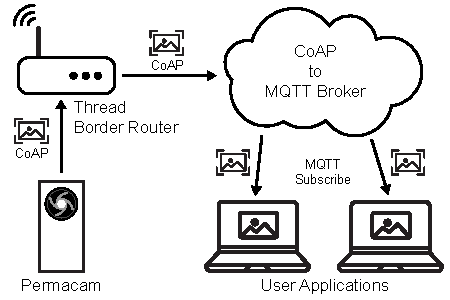
\includegraphics[width=\textwidth]{figs/capacity/arch}
        \caption{Harvesting and storage architecture}
    \end{subfigure}
    \begin{subfigure}{0.29\columnwidth}
        \centering
        \includegraphics[width=\textwidth,angle=90]{figs/capacity/permamote}
        \caption{Hardware}
    \end{subfigure}
    \caption{\normalfont The \name power supply architecture is informed by the
    findings in \cref{sec:store,sec:primary}. An
    LTO battery is recharged by a solar panel. When the battery is depleted,
    a primary-cell powers the system, providing reliability and avoiding
    intermittency.
    }
    %We believe this platform will run for 6-36 years for common
    %sensing tasks and indoor lighting conditions before the death of
    %the primary-cell. Even after the primary-cell expires,
    %the sensor node could continue to run intermittently on harvested energy.
\end{definefigure}

We implement the design principals discussed in \cref{sec:store,sec:primary}
in a new sensor called \name. The \name sensing platform
integrates a processor, BLE/802.15.4 radio, and various environmental, lighting,
and occupancy sensors. A picture
and system diagram of \name is shown in \cref{fig:permamote}. All hardware
and software for the platform is open source\footnote{\url{https://github.com/lab11/permamote/tree/master/hardware/permamote}}.\\

\vspace{-6pt}
\noindent
\textbf{Energy Harvesting and Storage.}
\name is powered by an energy harvesting front end that realizes the benefits
of using batteries. It uses the TI BQ25505 energy harvesting IC, which
harvests energy while monitoring both
rechargeable and backup energy stores,
switching between them at user-configurable voltages~\cite{bq25505}. A
20\,mAh (48\,mWh) LTO battery is charged by an 10.9\,cm\textsuperscript{2} amorphous
silicon solar panel~\cite{LTODatasheet, LTODatasheet2}. We limit the apparent
capacity of this battery to ensure
longer cycle lifetime as described in \cref{sec:battery}, but still have 24\,mWh of
energy storage, more than the capacity required to achieve the reliability and energy utilization
improvements described in \cref{sec:store}. For the backup energy
store, \name uses lithium primary-cells which can be configured to either one or two CR2032 coin
cells or a CR123A cell.
%Primary-cells provide 3-13x more density and 2-12x less
%leakage than a secondary-cell.
%making them more desirable than a single,
%large, pre-charged secondary-cell as the backup store~\cite{LTODatasheet,primary2032, primarycr123a}.
The output of the active battery
is boosted by a MAX17222 regulator, which features high conversion efficiency
(>90\%) at low output currents and operates down to 400\,mV~\cite{max17222}.\\
%We have the ability to monitor harvesting and system currents using
%the iCount method by sensing the voltage of
%the inductor used by the BQ25505 and MAX17222~\cite{duttaEnergy08}. The processor
%is also capable of gating all sensors from the main power supply to save
%power.\\

\vspace{-6pt}
\noindent
\textbf{Processor, Radio and Sensor Selection.}
In designing \name, we search for the newest and lowest power components.
%We feel that it may
To benefit other
platform builders, we document our component selections
along with their key performance metrics. A summary of these
components can be found in \cref{tab:components}.

We note our choice of the Nordic NRF52840 MCU over the more commonly used MSP430FR series
because of its higher efficiency in active mode while offering comparable sleep currents.
Specifically, it only draws 56\,\uA/MHz compared to over 100\,uA/MHz
for the MSP430. Unlike intermittent systems,
we do not rely on the FRAM present on the MSP430FR series chips. While
slightly more efficient
processors and radios exist than those found in the NRF52840,
we value the simplicity of an SoC-based design. \\

\vspace{-6pt}
\noindent
\textbf{Energy Benchmarks}.
The data presented in \cref{tab:components} are benchmarks taken
on the \name platform. We find that a BLE advertisement at 0\,dbm consumes
86\,\uJ and that sampling both light and color sensors and transmitting
them in a BLE advertisement consumes 586\,\uJ. Additionally, the entire system, including
the energy harvesting front end, consumes only 5.0\,\uW in deep sleep with RAM
retained and all sensors powered off. We use the energy numbers from \name as a basis
for our workloads to fairly compare against prior energy storage architectures.
%\subsection{Numerical Model}
%\label{impl:model}
%
%We develop a numerical model that simulates the behavior of energy harvesting
%systems in indoor environments. For this work, we've primarily focused on solar
%energy input, and have tailored the model to use solar energy traces. As
%mentioned, we use the Columbia EnHANTs irradiance traces
%\cite{margolies2015energy}. We process the traces, filling the few periods of
%missing data by copying from a week prior.
%
%The model operates at second granularity, and at each
%step, the amount of incoming energy is calculated based on the input irradiance
%and solar panel configuration. If the device has enough energy to turn on
%and perform the task from the specified workload it does so. If there is
%energy to spare after the task, the device will enter a low power sleep state.
%The model tallies the amount of successful and unsuccessful events that it
%was expected to complete, as well as the percentage of energy used out
%the energy that was available from the harvesting source. To estimate
%lifetime, the model attempts tasks for the totality of solar irradiance
%data present, then extrapolates primary-cell discharge to find its lifetime
%at empty. The one second granularity imposes some limitations, however
%we find that sensor node workloads are rarely more intensive.
%
%If the secondary store is not at capacity
%this incoming energy is stored
%
%If the device is online, it attempts to turn on
%if it has enough energy to do so, otherwise it remains offline and continues to
%fail performing its workload.  If the device is on, it perform tasks from its
%workload. It prioritizes using the energy from its rechargeable store, and if
%depleted, will either go offline or use energy from its primary-cell, if
%available. If it has energy to spare, it enters a low power sleep state. The
%model tallies the amount of successful and unsuccessful events that it was
%expected to complete, as well as the percentage of energy it used out of how
%much was available from the irradiance source. It also performs a linear fit on
%the primary state of charge to estimate lifetime, if applicable to the
%simulated device's configuration.
%
%This
%granularity also limits that of workloads to a second, but we argue
%that realistic sensor workloads are rarely more intensive \hl{cite}.


\placefigure[t]{fig:permamote}
